\documentclass[%
 reprint,
%superscriptaddress,
%groupedaddress,
%unsortedaddress,
%runinaddress,
%frontmatterverbose, 
%preprint,
%showpacs,preprintnumbers,
%nofootinbib,
%nobibnotes,
%bibnotes,
 amsmath,amssymb,
 aps,
%pra,
%prb,
%rmp,
%prstab,
%prstper,
%floatfix,
]{revtex4-1}

\usepackage{graphicx}% Include figure files
\usepackage{dcolumn}% Align table columns on decimal point
\usepackage{bm}% bold math
%\usepackage{hyperref}% add hypertext capabilities
%\usepackage[mathlines]{lineno}% Enable numbering of text and display math
%\linenumbers\relax % Commence numbering lines

%\usepackage[showframe,%Uncomment any one of the following lines to test 
%%scale=0.7, marginratio={1:1, 2:3}, ignoreall,% default settings
%%text={7in,10in},centering,
%%margin=1.5in,
%%total={6.5in,8.75in}, top=1.2in, left=0.9in, includefoot,
%%height=10in,a5paper,hmargin={3cm,0.8in},
%]{geometry}

\usepackage{cmap} % Поиск в PDF
\usepackage[T2A]{fontenc} % Кодировка
\usepackage[utf8]{inputenc} % Кодировка исходного текста
\usepackage[english, russian]{babel} % Локализация и переносы
\frenchspacing % Более тонкая настройка пробелов 
\usepackage{multirow}
\usepackage[warn]{mathtext}
\usepackage{amssymb}
\usepackage{ dsfont }

% Переопределение англоязычного начертания каппа, фи и эпсилон, 
% а также знаков сравнения
\renewcommand{\epsilon}{\ensuremath{\varepsilon}}
\renewcommand{\phi}{\ensuremath{\varphi}} 
\renewcommand{\kappa}{\ensuremath{\varkappa}}
\renewcommand{\le}{\ensuremath{\leslant}}
\renewcommand{\leq}{\ensuremath{\leqslant}}
\renewcommand{\ge}{\ensuremath{\geslant}}
\renewcommand{\geq}{\ensuremath{\geqslant}}
\renewcommand{\emptyset}{\ensuremath{\varnothing}}

\usepackage{textcomp} 
\usepackage{indentfirst} % Красная строка
\usepackage{amsmath} % Текст в формулах
\usepackage{graphicx} % Графика
\DeclareGraphicsExtensions{.pdf,.png,.jpg}
\usepackage{pgfplots}
\pgfplotsset{compat=1.13}

%\usepackage{times}

\begin{document}

\title{Эффект Холла в полупроводниках}
\thanks{3.3.4}

\author{Иван Едигарьев,}
\affiliation{
 Московский Физико-Технический Институт\\
 Факультет Общей и Прикладной Физики, 526т\\
}
%\date{\today}

\begin{abstract}
Цель работы: 1) измерение подвижности и концентрации носителей заряда в полупроводниках.

В работе используются: электромагнит с источником питания, амперметр, миллиамперметр, милливеберметр, реостат, цифровой вольтметр, источник питания (1,5~B), образцы легированного германия.

\end{abstract}

\pacs{Valid PACS appear here}% PACS, the Physics and Astronomy
                             % Classification Scheme.
%\keywords{Suggested keywords}%Use showkeys class option if keyword
                              %display desired
\maketitle

%\tableofcontent

\section{\label{sec:level1}Теоретическая справка.}

Значение для ЭДС Холла даётся выражением: 
\\

\begin{equation}\label{1}
    {\mathscr{E}}_x = - \frac{IB}{nea} = - R_x \frac{IB}{a}
\end{equation}

Константа $R_x$ называется постоянной Холла и даётся выражением:

\begin{equation}\label{2}
    R_x = \frac{1}{ne}
\end{equation}

Также будет полезным записать выражение для значения удельной электрической проводимости:

\begin{equation}\label{3}
    \sigma = enb
\end{equation}

\section{\label{sec:level1}Экспериментальная установка.}

 Электрическая схема установки для измерения ЭДС Холла представлена на рис. 1.
 
    В зазоре электромагнита (рис. 1а) создаётся постоянное магнитное поле, величину которого можно менять с помощью регулятора $R_1$ источника питания электромагнита. Ток питания электромагнита измеряется амперметром $A_1$. Разъём $K_1$ позволяет менять направление тока в обмотках электромагнита.
    
    Градуировка магнита проводится при помощи милливеберметра. Описание милливеберметра и правила работы с ним приведены на с. 148.[1]
    
    Образец из легированного германия, смонтированный в специальном держателе (рис. 1б), подключается к источнику питания ($\sim$ 1,5 В).

При замыкании ключа $K_2$ вдоль длинной стороны образца течёт ток, величина которого регулируется реостатом $R_1$ и измеряется миллиамперметром $A_2$.
\\
\\
\\
\\
\\
\\
\\
\\
\\
\\
\\
\\
\\
\\
\\
\\
\\
\\
\\
\\
\\
\\
\\
\\
   В образце с током, помещённом в зазор электромагнита, между контактами 3 и 4 возникает разность потенциалов $U_{34}$ , которая измеряется с помощью цифрового вольтметра.
   
   Иногда контакты 3 и 4 вследствие неточности подпайки не лежат на одной эквипотенциали, и тогда напряжение между ними связано не только с эффектом Холла, но и с омическим падением напряжения, вызванным протеканием основного тока через образец. Измеряемая разность потенциалов при одном направлении магнитного поля равна сумме ЭДС Холла и омического падения напряжения, а при другом — их разности. В этом случае ЭДС Холла $\mathscr{E}_x$ может быть определена как половина алгебраической разности показаний вольтметра, полученных для двух противоположных направлений магнитного поля в зазоре. Знак измеряемого напряжения высвечивается на цифровом табло вольтметра.

Можно исключить влияние омического падения напряжения иначе, если при каждом токе через образец измерять напряжение между точками 3 и 4 в отсутствие магнитного поля. При фиксированном токе через образец это дополнительное к ЭДС Холла напряжение $U_0$ остаётся неизменным. От него следует (с учётом знака) отсчитывать величину ЭДС Холла:
\begin{equation}\label{4}
    \mathscr{E}_x = U_{34} \pm U_0
\end{equation}
При таком способе измерения нет необходимости проводить повторные измерения с противоположным направлением магнитного поля.
     По знаку $\mathscr{E}_x$ можно определить характер проводимости — электронный или дырочный. Для этого необходимо знать направление тока в образце и направление магнитного поля.
     
     Измерив ток $I$ в образце и напряжение $U_{35}$ между контактами 3 и 5 в отсутствие магнитного поля, можно, зная параметры образца, рассчитать проводимость материала образца по формуле
\begin{equation}\label{5}
    \sigma = \frac{I L_{35}}{U_{35} a l}
\end{equation}    
где $L_{35}$ — расстояние между контактами 3 и 5, $a$ — толщина образца, $l$ — его ширина.
   
\section{\label{sec:level1}Задание.}

В работе предлагается исследовать зависимость ЭДС Холла от величины магнитного поля при различных токах через образец для определения константы Холла; определить знак носителей заряда и проводимость материала образца.\\
 1. Подготовьте приборы к работе.\\
 2. Проверьте работу цепи питания образца. Ток через образец не должен превышать 1 мА.\\
 3. Проверьте работу цепи магнита. Определите диапазон изменения тока через магнит.\\
 4. Прокалибруйте электромагнит — опред елите связь между индукцией $B$ магнитного поля в зазоре электромагнита и током $I_{\text{м}}$ через обмотки магнита. Для этого с помощью милливеберметра снимите зависимость магнитного потока Ф, пронизывающего пробную катушку, находящуюся в зазоре, от тока $I_{\text{м}}$ ($\text{Ф}~=~BSN)$. Значение $SN$ (произведение площади сечения контура катушки на число витков в ней) указано на держателе катушки.\\
5. Проведите измерение ЭДС Холла. Для этого вставьте образец в зазор выключенного электромагнита и определите напряжение $U_0$ между холловскими контактами 3 и 4 при минимальном токе через образец ($\backsimeq$ 0,2 мА). Это напряжение $U_0$ вызвано несовершенством контактов 3, 4 и при фиксированном токе через образец остаётся неизменным. Значение $U_0$ с учётом знака следует принять за нулевое.


   Включите электромагнит и снимите зависимость напряжения $U_{34}$ от тока $I_{\text{м}}$ через обмотки магнита при фиксированном токе через образец.
   
   Проведите измерения $U_{34} = f(I_{\text{м}})$ при постоянном токе через образец для 6-8 его значений в интервале 0,2-1 мА. При каждом новом значении тока через образец величина $U_0$ будет иметь своё значение.
   
   При максимальном токе через образец ($\backsimeq$ 1 мА) проведите измерения $U_{34} = f(I_{\text{м}})$ при другом направлении магнитного поля.\\
 6. Определите знак носителей в образце. Для этого необходимо знать направление тока через образец, направление магнитного поля и знак ЭДС Холла.
   
   Направление тока в образце показано знаками «+» и «—» на рис. 1. Направление тока в обмотках электромагнита при установке разъёма $K_1$ в положение I показано стрелкой на торце магнита.
   
   Зарисуйте в тетради образец. Укажите на рисунке направления тока, магнитного поля и отклонение носителей. По знаку ($\pm$) на клеммах цифрового вольтметра определите характер проводимости.\\
 7. Для определение удельной проводимости удалите держатель с образцом из зазора. Подключите к клеммам «$H_x$» и «$L_x$» вольтметра потенциальные концы 3 и 5. Измерьте падение напряжения между ними при токе через образец 1 мА.\\
 8. Запишите характеристики приборов и параметры образца $L_{35}$, $a$, $l$, указанные на держателе.\\
 \begin{center}
  Обработка результатов
\end{center}
1. Постройте график зависимости $B = f(I_{\text{м}})$\\
 2. Рассчитайте ЭДС Холла по формуле (4) и постройте на одном листе семейство характеристик $\mathscr{E}_x = f(B)$ при разных значениях тока $I$ через образец. Определите угловые коэффициенты $k(I) = {\Delta{\mathscr{E}_x}}/{\Delta{B}}$ полученных прямых. 
 
Постройте график $k = f(I)$. Рассчитайте угловой коэффицие прямой и по формуле (1) определите величину постоянной Холла $R_{X}$. Рассчитайте концентрацию $n$ носителей тока в образце по формуле (2).
   
   Оцените погрешность результата и сравните результат с табличным.\\
 3. Рассчитайте удельную проводимость $\sigma$ материала образца по формуле (5). 
 
 Используя найденные значения концентрации $n$ и проводимости $\sigma$, с помощью формулы (3) вычислите подвижность $b$ носителей тока в общепринятых для этой величины внесистемных единицах: размерность напряжённости электрического поля [$E$]~=~[$U/L$]~=~В/см, размерность скорости [$v$] = см/с, поэтому размерность подвижности [$b$] = $\text{см}^2$/($B \cdot c$).
 
Оцените погрешности и сравните результаты с табличными.

\section{\label{sec:level1}Данные.}

Взглянем на данные измерений, а именно построим график $B~=~f(I_m)$. Заметим, что линейность отклика графика отвергается начиная с 4-5 измерения. Данный эффект можно обьяснить так называемым эффектом насыщения железа, то есть резким спадом магнитной проницаемости при больших значениях магнитного поля порядка $1~T$, что и легко заметить в данном эксперименте.

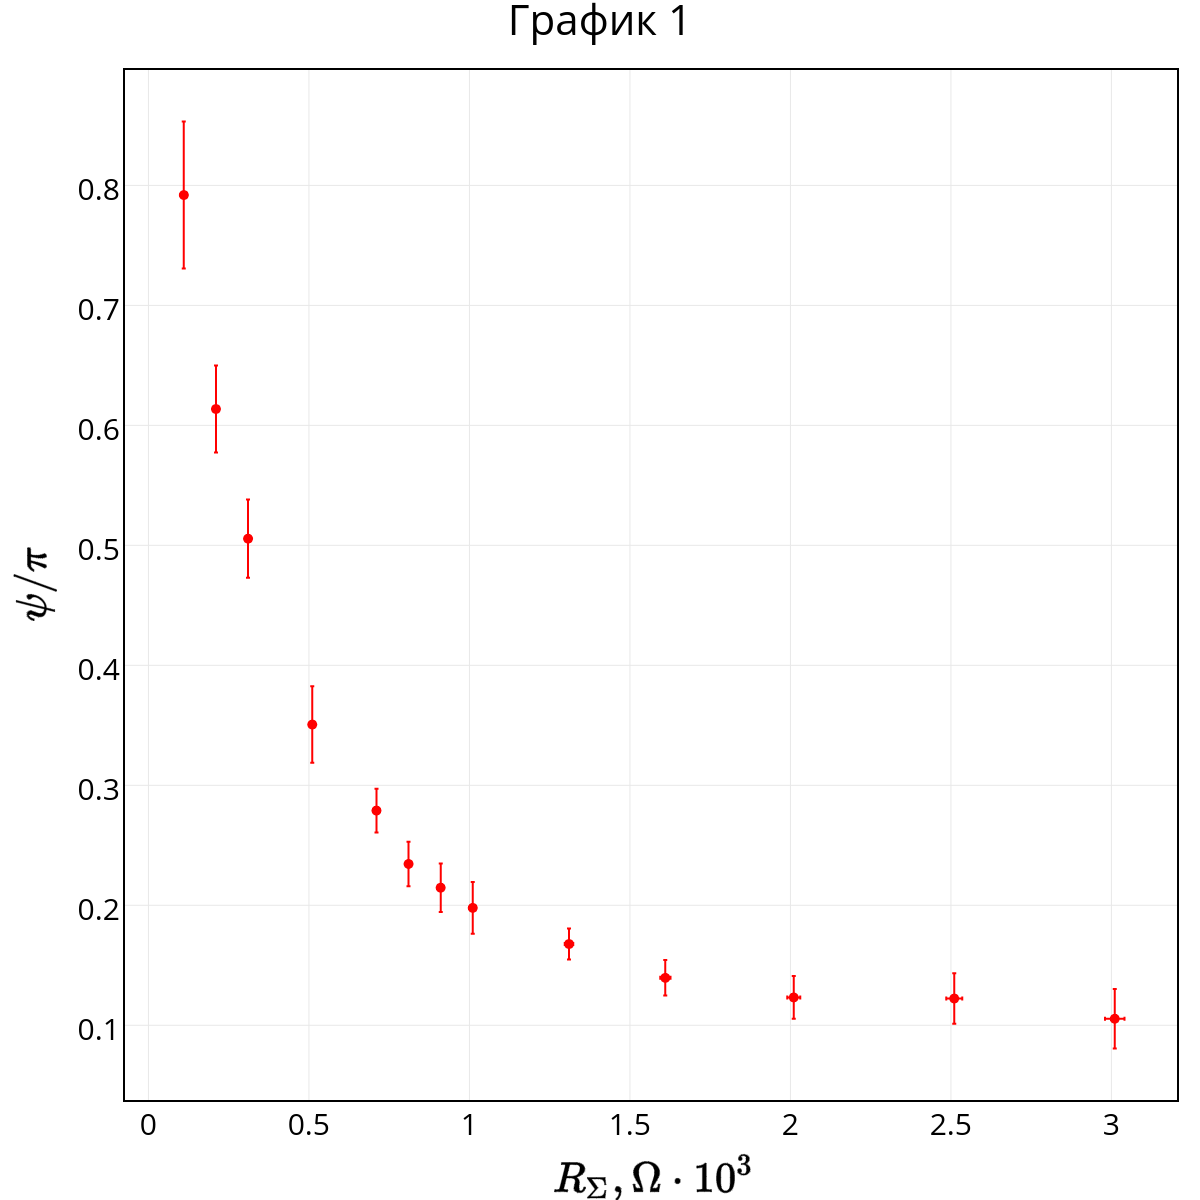
\includegraphics[scale = 0.20]{my_plot1.png}

Эксперимент осуществлялся таким образом, что дальнейшие измерения ЭДС Холла проводились при тех же значениях тока, что и при построении зависимости $B~=~f(I_m)$, это и будет являться калибровкой электромагнита.

Далее построим графики по всем семействам характеристик $\mathscr{E}_x = f(B)$, измерения проводились при 8 различных значениях $I$ - тока через образец. Заранее выровняем значения на $U_0$ в каждой серии, $U_0$ было измерено заранее.

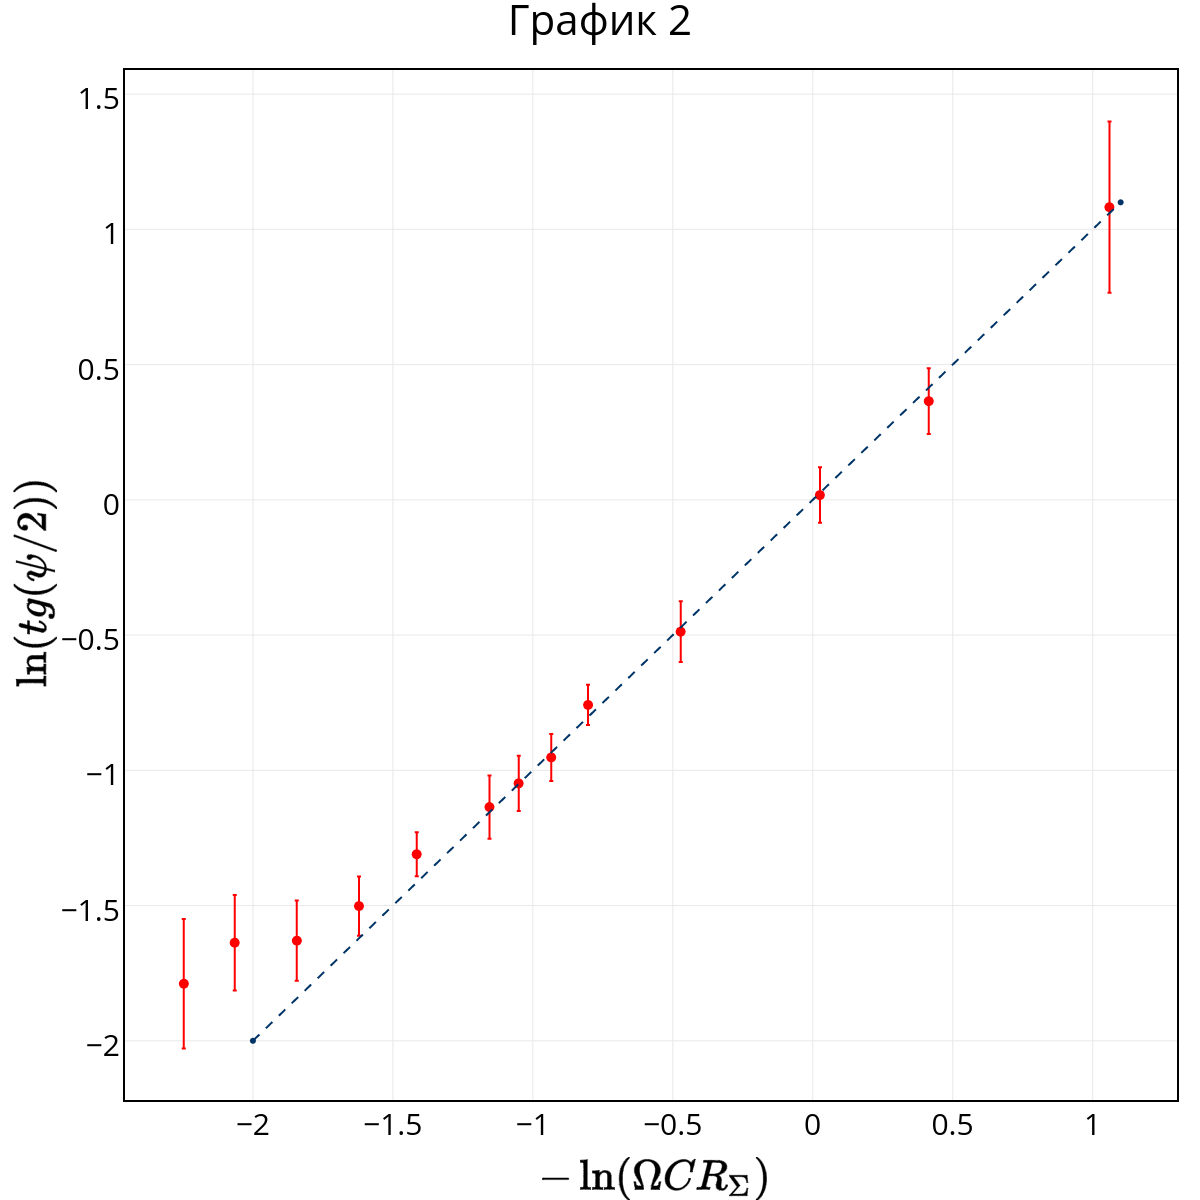
\includegraphics[scale = 0.20]{my_plot2.png}

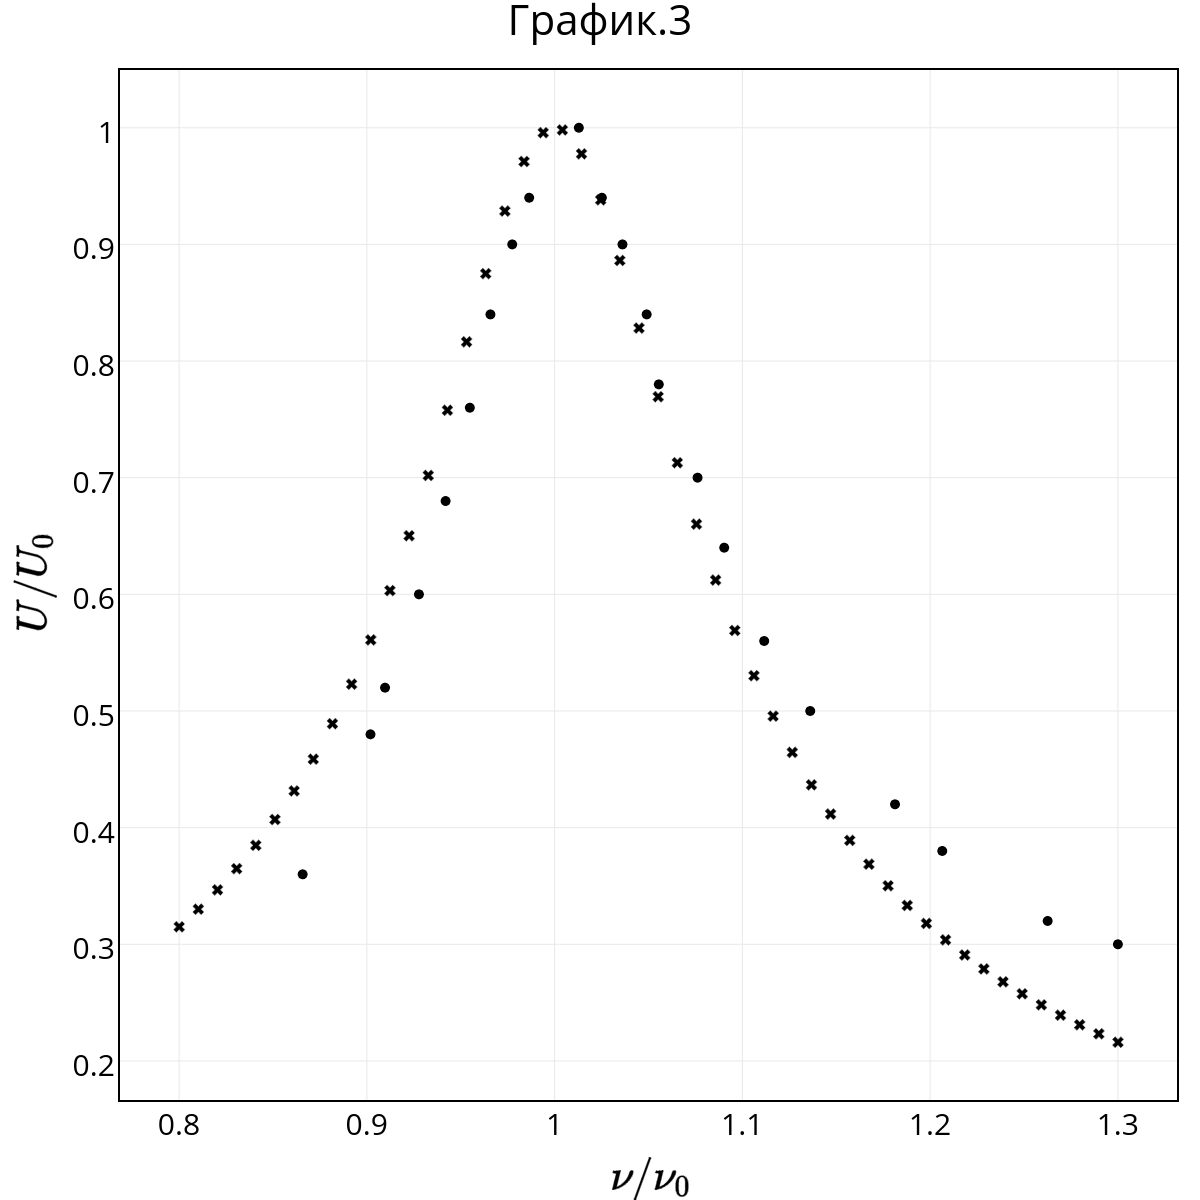
\includegraphics[scale = 0.20]{my_plot3.png}

Как видим на всех сериях наблюдается устойчивый линейный отклик, в отличии от $B~=~f(I_m)$. Систематическая погрешность составляет не более процента от измеряемых величин напряжения и магнитного поля. 

Также дополнительно к 8 серии на величине тока $I_m=1~A$ через обмотки магнита было проведено измерение при другом направлении магнитного поля. Для каждой из этих серий заранее было измерено показание $U_0$, в предположении того, что две серии будут идентичны с учётом нормировки на $U_0$ и изменение знака $U_{34}$. Построим график разности модулей значений в этих двух сериях.

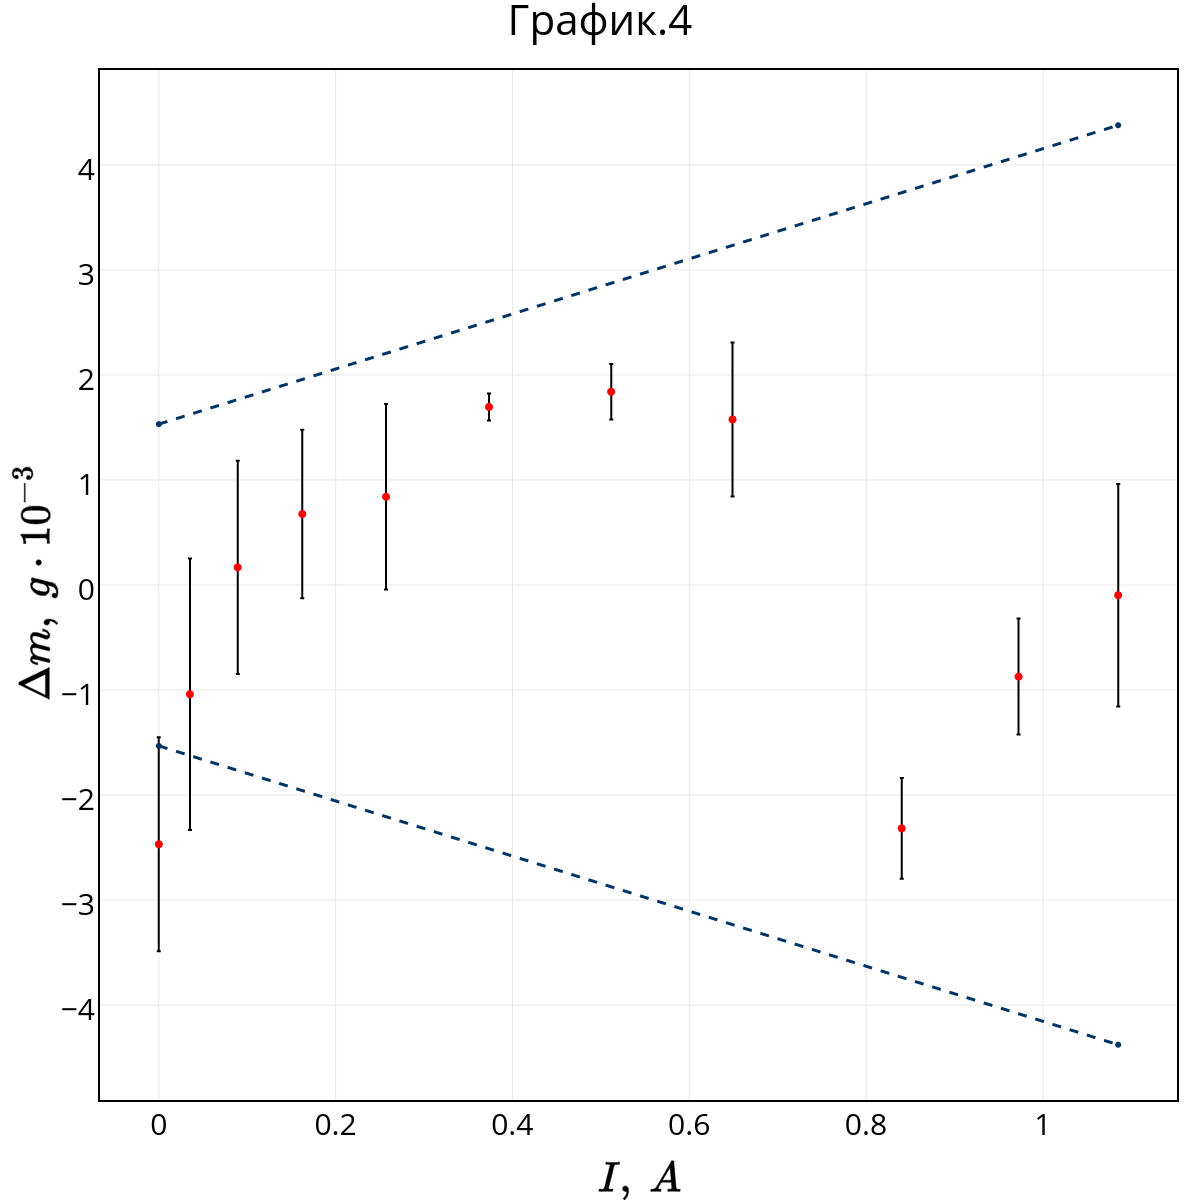
\includegraphics[scale = 0.20]{my_plot4.png}

Как видим имеет место довольно странный разброс, не лежащий в пределах измерений $U_0$ для двух серий. В дальнейшем не будем использовать значения $U_0$ и построим модель со свободным членом, это не повлияет на итоговое значение коэффициента пропорциональности в зависимости $\mathscr{E}_x = f(B)$.

Построим обычный метод наименьших квадратов. Усложнение метода построения регрессии не требуется в связи с опять таки хорошо заметным линейным откликом и малыми гомоскедастичными систематическими ошибками. 

1) Метод наименьших квадратов (least squares):
$$ \beta = \text{argmin}_{\beta, k}(\sum_i^n (y_i - k x_i - \beta)^2) $$

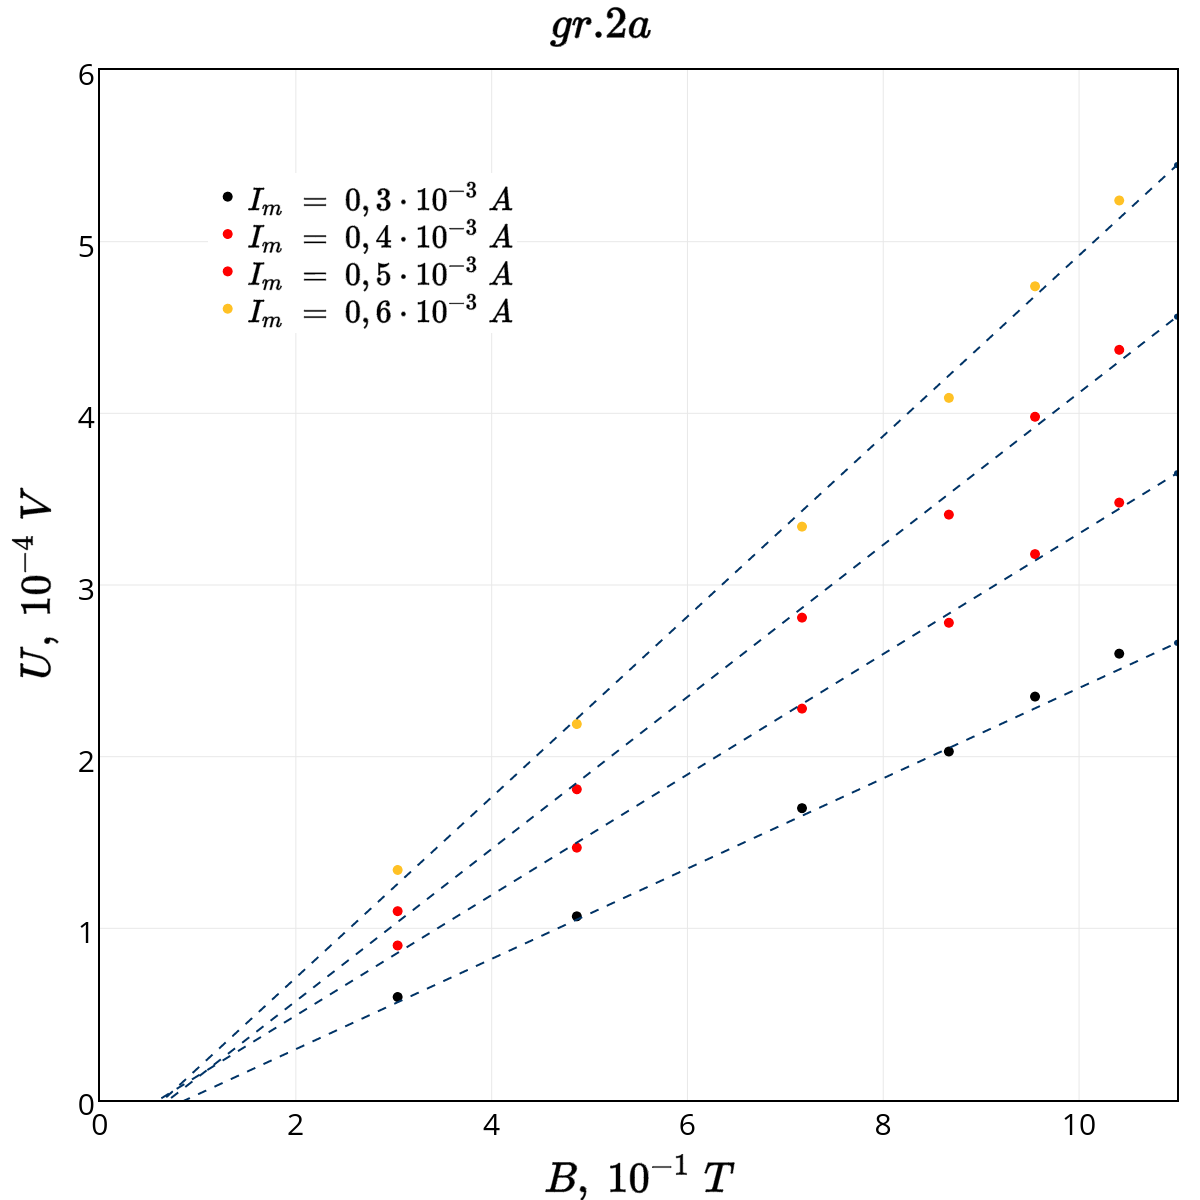
\includegraphics[scale = 0.20]{my_plot2a.png}\\

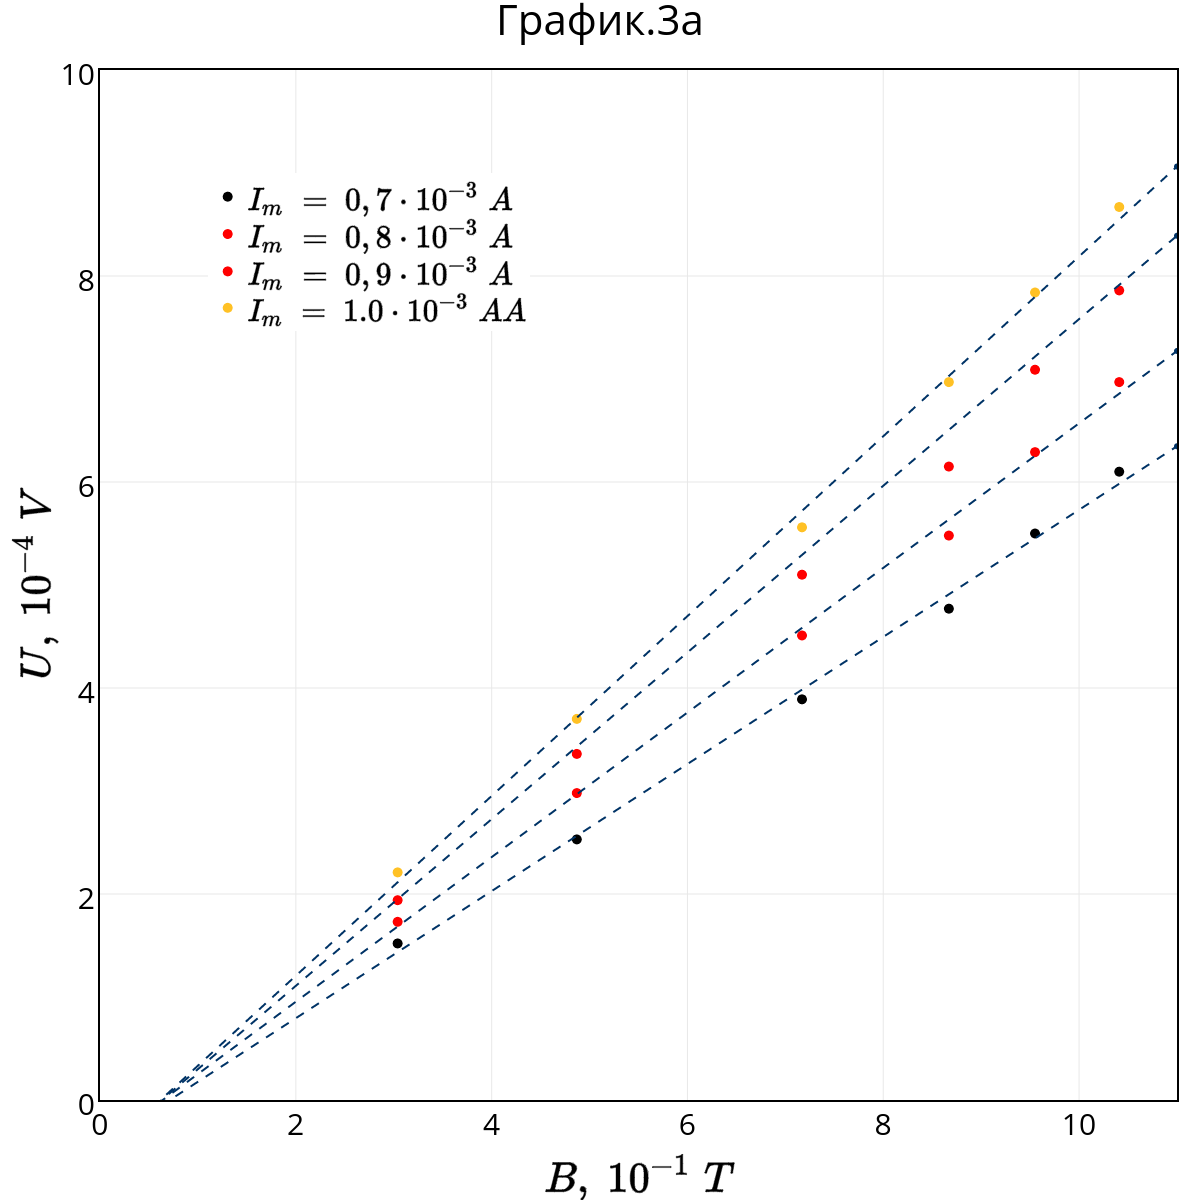
\includegraphics[scale = 0.20]{my_plot3a.png}

В итоге получим решение задачи регресии с данными коэффициентами при значениях магнитного поля:

\begin{center}
\begin{tabular}{|c|*{8}{c|}}
\hline
{$I,~10^{-4}~A$} & $3$ &  $4$ & $5$ & $6$ & $7$ & $8$ & $9$ & $10$  \\
\hline
{$k,~10^{-6}~V\cdot T^{-1}$} & $268$ &  $351$ & $443$ & $526$ & $617$ & $702$ & $791$ & $873$ \\
\hline
{$\sigma_k,~10^{-6}~V\cdot T^{-1}$} & $6$ &  $7$ & $13$ & $17$ & $18$ & $17$ & $20$ & $18$\\
\hline
{$\beta, 10^{-6}~V$} & $-23$ &  $-21$ & $-31$ & $-34$ & $-44$ & $-45$ & $-51$ & $-54$ \\
\hline
\end{tabular}
\end{center}

Построим теперь уже график зависимости $k = f(I)$.\\

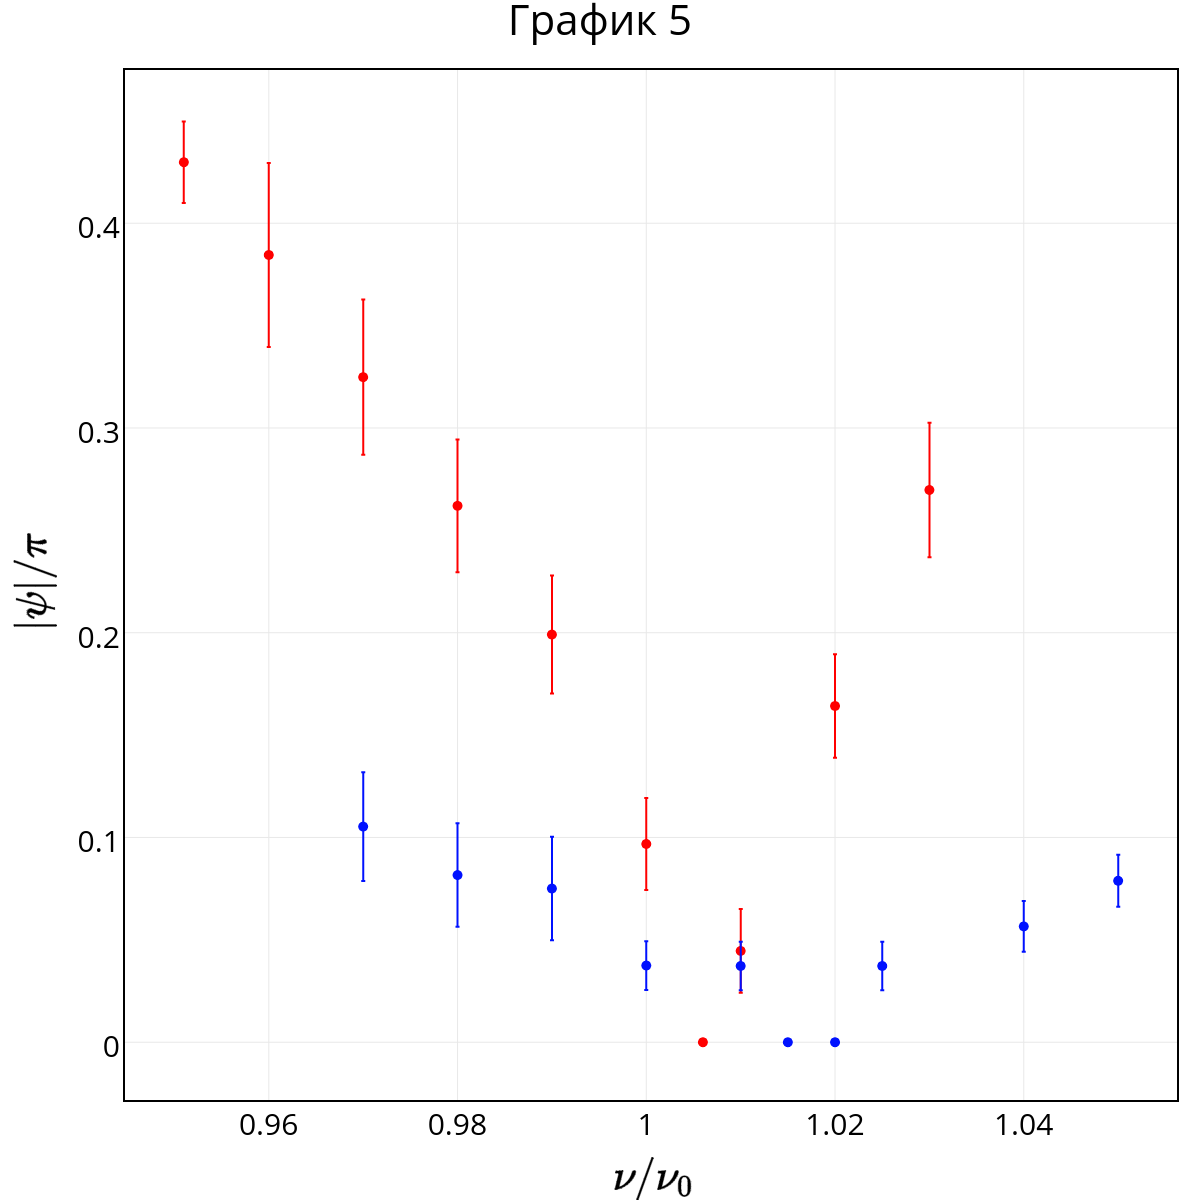
\includegraphics[scale = 0.20]{my_plot5.png}

Теперь построим аналогичную регрессию только в модели уже без свободного члена, исходная физическая модель зависимости $k = f(I)$ предполагается строго линейной. 

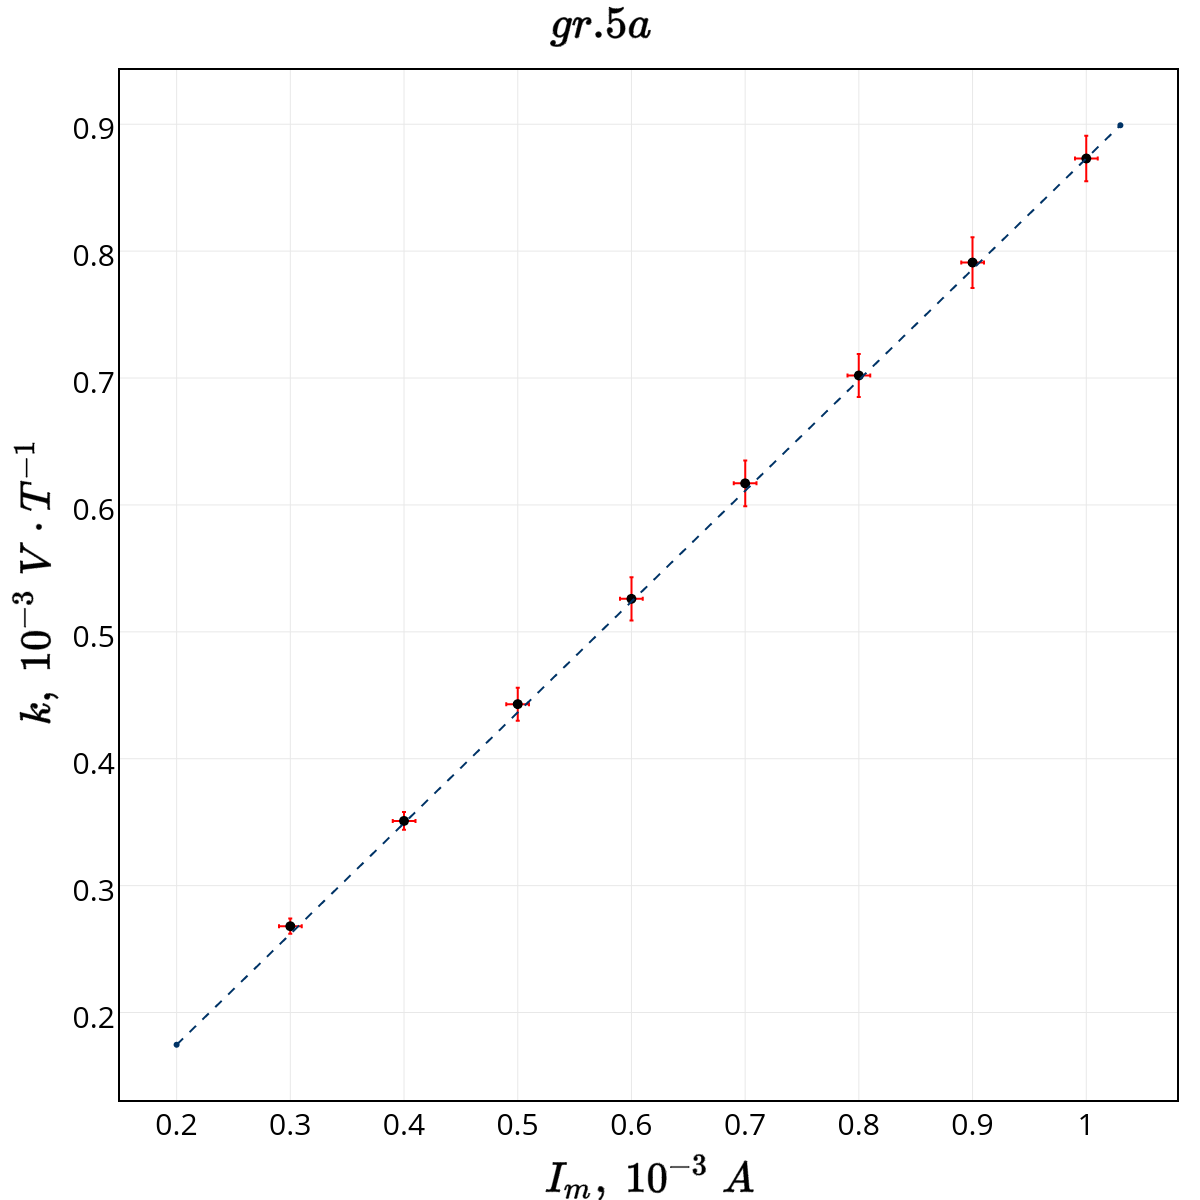
\includegraphics[scale = 0.20]{my_plot5a.png}\\
\\
\newpage
Итоговое значение получим в виде:

$$\boxed{\frac{R_x}{a} = (893 \pm 13^{stat} \pm 38^{syst}) \times 10^{-3}~V \cdot T^{-1} \cdot A^{-1}}$$

Теперь определим величину постоянной Холла $R_x$ по формуле (1), а также концентрацию $n$ носителей тока в образце по формуле (5):

$$\boxed{R_x = (893 \pm 13^{stat} \pm 47^{syst}) \times 10^{-6}~V \cdot m \cdot T^{-1} \cdot A^{-1}}$$
$$\boxed{n = (698 \pm 11^{stat} \pm 37^{syst}) \times 10^{19} \cdot m^{-3}}$$

Также по измеренным в пункте 5. данным определим величину и ошибку проводимости $\sigma$ образца с помощью формулы (3):

$$\boxed{\sigma = (390 \pm 12^{syst})~Ohm\cdot m^{-1}}$$

И окончательно вычислим значение и оценим ошибку подвижности $b$ носителей тока:

$$\boxed{b = (3482 \pm 55^{stat} \pm 456^{syst})~cm^2 \cdot V^{-1} \cdot s^{-1}}$$

Приведём табличное значение подвижности для электронного типа проводимости германия:

$$\boxed{b_{\text{Ge}} = 3800~cm^2 \cdot V^{-1} \cdot s^{-1}}$$

Как видим, результаты согласуются с точностью до одного стандартного отклонения.

\newpage
\section{\label{sec:level1}Тип носителей.}

Изобразим образец, укажем направление тока, магнитного поля и знак ЭДС Холла:
\\
\\
\\
\\
\\
\\
\\
\\
\\
\\
\\
\\
\\
\\
\\
\\
\\

Тип продимости в нашем случае будет элетронным. 

\section{\label{sec:level1}Ссылки.}
[1] - Лабораторный практикум по общей физике. Электричество и магнетизм. МФТИ, 2007. ISBN 5-7417-0204-x (T. 2)

LS - scipy.optimize.curve\_fit

Весь процесс обработки данных можно проделать в открытом репозитории:

\href{github.com/heyfaraday/labs_3sem/tree/master/3.1.2}{github.com/heyfaraday/labs\_3sem/tree/master/3.3.4}
\end{document}

